\documentclass[journal]{IEEEtran}
\usepackage[a5paper, margin=10mm]{geometry}
%\usepackage{lmodern} % Ensure lmodern is loaded for pdflatex
\usepackage{tfrupee} % Include tfrupee package


\setlength{\headheight}{1cm} % Set the height of the header box
\setlength{\headsep}{0mm}     % Set the distance between the header box and the top of the text


%\usepackage[a5paper, top=10mm, bottom=10mm, left=10mm, right=10mm]{geometry}

%
\setlength{\intextsep}{10pt} % Space between text and floats

\makeindex


\usepackage{cite}
\usepackage{amsmath,amssymb,amsfonts,amsthm}
\usepackage{algorithmic}
\usepackage{graphicx}
\usepackage{textcomp}
\usepackage{xcolor}
\usepackage{txfonts}
\usepackage{listings}
\usepackage{enumitem}
\usepackage{mathtools}
\usepackage{gensymb}
\usepackage{comment}
\usepackage[breaklinks=true]{hyperref}
\usepackage{tkz-euclide} 
\usepackage{listings}
\usepackage{multicol}
\usepackage{xparse}
\usepackage{gvv}
%\def\inputGnumericTable{}                                 
\usepackage[latin1]{inputenc}                                
\usepackage{color}                                            
\usepackage{array}                                            
\usepackage{longtable}                                       
\usepackage{calc}                                             
\usepackage{multirow}                                         
\usepackage{hhline}                                           
\usepackage{ifthen}                                               
\usepackage{lscape}
\usepackage{tabularx}
\usepackage{array}
\usepackage{float}
\usepackage{ar}
\usepackage[version=4]{mhchem}


\newtheorem{theorem}{Theorem}[section]
\newtheorem{problem}{Problem}
\newtheorem{proposition}{Proposition}[section]
\newtheorem{lemma}{Lemma}[section]
\newtheorem{corollary}[theorem]{Corollary}
\newtheorem{example}{Example}[section]
\newtheorem{definition}[problem]{Definition}
\newcommand{\BEQA}{\begin{eqnarray}}
\newcommand{\EEQA}{\end{eqnarray}}

\theoremstyle{remark}


\begin{document}
\bibliographystyle{IEEEtran}
\onecolumn

\title{12.249}
\author{INDHIRESH S- EE25BTECH11027}
\maketitle


\renewcommand{\thefigure}{\theenumi}
\renewcommand{\thetable}{\theenumi}

\textbf{Question}. A plane contains the following three points: $\Vec{P}(2, 1, 5), \Vec{Q}(-1, 3, 4)$ and $\Vec{R}(3, 0, 6)$. The vector perpendicular to the above plane can be represented as\\
\textbf{Solution}:\\
Let us solve the given equation theoretically and then verify the solution computationally. \\
Given points are:
\begin{align}
 \Vec{P}=\myvec{2\\1\\5}\;\;,\Vec{Q}=\myvec{-1\\3\\4}\;\;and\;\;\Vec{R}=\myvec{3\\0\\6}
\end{align}
The equation of plane through the points $\Vec{P}$,$\Vec{Q}$ and $\Vec{R}$ can be given as
\begin{align}
\myvec{\Vec{P}&\Vec{Q}&\Vec{R}}^T\Vec{n}=\myvec{1\\1\\1}
\end{align}
Where $\Vec{n}$ is the normal to the plane
\begin{align}
\myvec{2&-1&3\\1&3&0\\5&4&6}^T \Vec{n}=\myvec{1\\1\\1}
\end{align}
\begin{align}
    \myvec{2&1&5\\-1&3&4\\3&0&6} \Vec{n}=\myvec{1\\1\\1}
\end{align}
Now forming the augmented matrix and performing row operations
\begin{align}
   \augvec{3}{2}{2&1&5&1\\-1&3&4&1\\3&0&6&1}\xleftrightarrow{R_2\longleftarrow -R_2} \augvec{3}{2}{2&1&5&1\\1&-3&-4&-1\\3&0&6&1}
\end{align}

\begin{align}
  \augvec{3}{2}{2&1&5&1\\1&-3&-4&-1\\3&0&6&1}\xleftrightarrow[R_1\longleftarrow R_1-2R_2]{R_3\longleftarrow R_3-3R_2}\augvec{3}{2}{0&7&13&3\\1&-3&-4&-1\\0&9&18&4}
\end{align}

\begin{align}
\augvec{3}{2}{0&7&13&3\\1&-3&-4&-1\\0&9&18&4}\xleftrightarrow{R_3\longleftarrow 7R_3-9R_1}\augvec{3}{2}{0&7&13&3\\1&-3&-4&-1\\0&0&9&1}
\end{align}

\begin{align}
\augvec{3}{2}{0&7&13&3\\1&-3&-4&-1\\0&0&9&1}\xleftrightarrow[R_1\longleftarrow \frac{1}{7}R_1]{R_3\longleftarrow \frac{1}{9}R_3} \augvec{3}{2}{0&1&\frac{13}{7}&\frac{3}{7}\\1&-3&-4&-1\\0&0&1&\frac{1}{9}}
\end{align}

\begin{align}
 \augvec{3}{2}{0&1&\frac{13}{7}&\frac{3}{7}\\1&-3&-4&-1\\0&0&1&\frac{1}{9}} \xleftrightarrow[R_2\longleftarrow R_2+4R_3]{R_1\longleftarrow R_1-\frac{13}{7}R_3}\augvec{3}{2}{0&1&0&\frac{2}{9}\\1&-3&0&-\frac{5}{9}\\0&0&1&\frac{1}{9}} 
\end{align}

\begin{align}
 \augvec{3}{2}{0&1&0&\frac{2}{9}\\1&-3&0&-\frac{5}{9}\\0&0&1&\frac{1}{9}}\xleftrightarrow{R_2\longleftarrow R_2+3R_1}  \augvec{3}{2}{0&1&0&\frac{2}{9}\\1&0&0&\frac{1}{9}\\0&0&1&\frac{1}{9}}
\end{align}

\begin{align}
 \augvec{3}{2}{0&1&0&\frac{2}{9}\\1&0&0&\frac{1}{9}\\0&0&1&\frac{1}{9}}\xleftrightarrow{R_2\longleftrightarrow R_1} \augvec{3}{2}{1&0&0&\frac{1}{9}\\0&1&0&\frac{2}{9}\\0&0&1&\frac{1}{9}}
\end{align}
The equation of plane can be given as:
\begin{align}
   \myvec{1&2&1}\Vec{x}=9
\end{align}
Normal of the plane is:
\begin{align}
   \Vec{n}=\myvec{1\\2\\1}  
\end{align}
This normal vector is perpendicular to the plane.\\\\
From the figure it is clearly verified that the theoretical solution matches with the computational solution.\\
\begin{figure}[h]
    \centering
    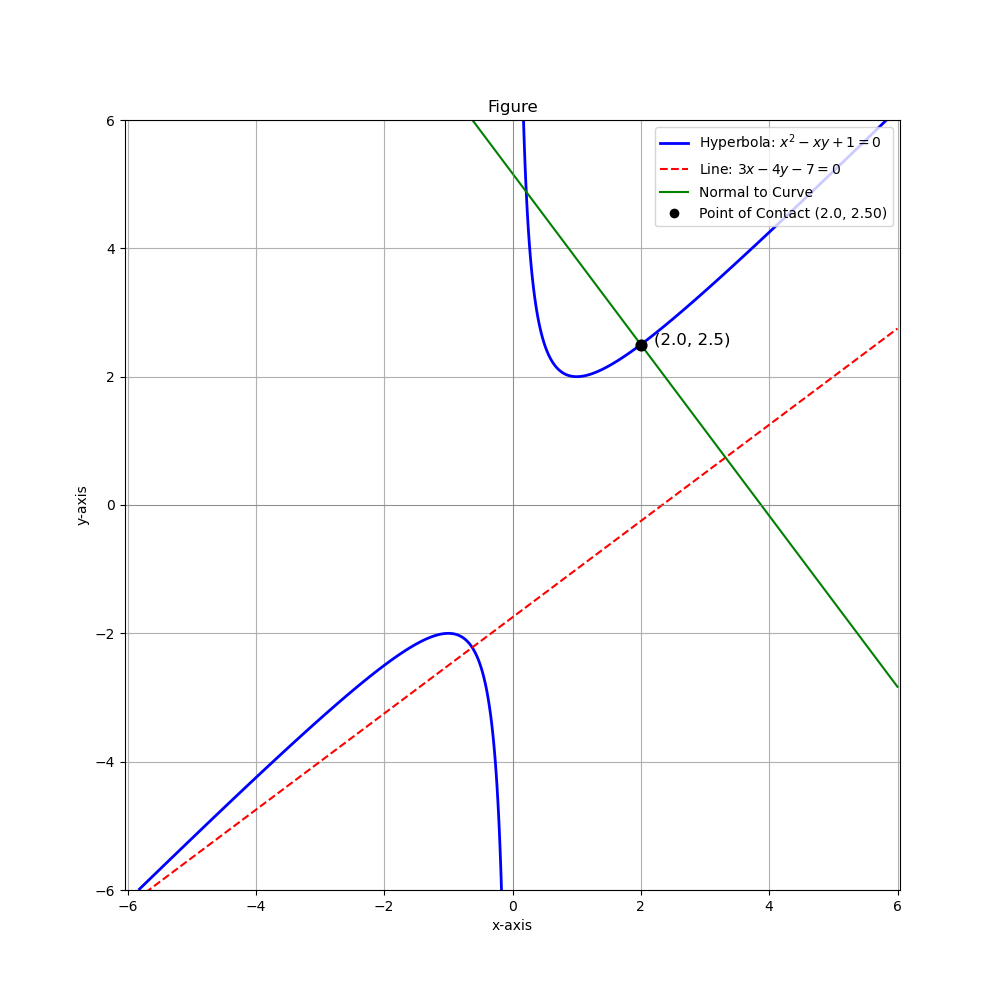
\includegraphics[height=0.5\textheight, keepaspectratio]{figs/figure1.png}
    \label{figure_1}
\end{figure}

\end{document}